% !TeX root = ../main.tex

\chapter{面向语音交互的多模态情感描述大模型方法研究}

在语音情绪分析领域,准确地识别并生成情感描述信息对于提升用户体验至关重要。近年来,随着大语言模型和深度学习技术的发展,多模态模型的应用逐渐成为该领域的研究热点。多模态情感描述生成不仅要求模型能够理解语音中的情感信息,还要能够将这一信息通过文本形式准确地传达给用户。为了实现这一目标,本文提出了一种面向语音交互的多模态情感描述大模型 SEMO-LLM,旨在提高情感描述生成的准确性和表达能力。

本文提出的 SEMO-LLM 模型结构由语音处理模块、稀疏桥接 Transformer 模块和大模型情感描述生成模块三部分组成。语音处理模块负责对原始语音数据进行预处理、特征提取和情感标签生成,从而为后续模型的训练提供高质量的语音数据。稀疏桥接 Transformer 模块通过稀疏自注意力和交叉注意力机制实现语音和文本特征的融合与对齐,确保多模态数据在情感特征上的一致性表达。最后,情感描述生成模块利用大语言模型生成符合语音语境的情感描述文本。

在实验部分,本文对 IEMOCAP 和 MELD 数据集了情感描述标注,并针对这两个数据进行训练与评估。通过与多种基线模型的对比实验,本文提出的多模态情感描述大模型 SEMO-LLM 在多个评估指标上取得了显著的提升,验证了该模型在情感描述生成任务中的有效性。特别是在 BLEU-1、BLEU-4、ROUGE-L 和 BERTScore 等评估指标上,本文模型相较于其他基线模型均展现出了更强的情感描述能力。此外为了验证 SEMO-LLM 模型结构的有效性,本文还进行了消融实验,结果表明本文提出的模型在音频编码器、桥接网络和文本解码器的组合上均取得了优于基线模型的表现。

\section{任务目标}

随着语音情绪分析的深入研究,现有的大部分情感分析方法普遍依赖于情感标签分类,存在较为粗糙的情感标签预测问题。在现有的情感分析框架中,情感标签通常仅能反映语音中的情感种类,而缺乏细粒度的情感表达。现有的开源语音情绪分析数据集如 IEMOCAP 和 MELD,主要关注情感分类任务,缺乏对情感描述的细致建模。因此本研究的第一步任务是对现有公开数据集进行情感描述标注扩充。通过利用大语言模型进行情感标签的预标注,并结合人工修正的方式,精细化标注现有数据集中的情感信息,这一过程将为后续模型训练提供高质量的情感标注数据。

由于语音情感描述数据的缺乏,现有的大部分语音情绪分析模型都是直接做固定的情感分类任务,而缺乏对情感描述生成的深入研究。因此,本研究的第二步任务是设计一种多模态情感描述大模型 SEMO-LLM,旨在通过语音和文本两种模态的深度融合,实现高精度情感识别与提示信息生成。该模型将通过语音处理模块、稀疏桥接 Transformer 模块和大模型情感描述生成模块三个部分组成,实现语音情感特征的提取、多模态特征的融合和情感描述文本的生成。其中,大模型情感描述生成模块将基于第三章所训练的心理大语言模型 PsycoLLM 作为底座,实验结果表明,相比在通用的大模型上进行训练,基于心理大语言模型的情感描述生成模型在情感描述任务上取得了更好的效果。

\section{多模态情感描述大模型结构设计}

\subsection{模型整体结构}

为了解决上面提到的问题,本文提出的多模态情感描述大模型 SEMO-LLM 的流程图和模型结构细节图分别如图 ~\ref{fig:work2-workflow} 和图 ~\ref{fig:work2-architecture} 所示,SEMO-LLM 由语音处理模块、稀疏桥接 Transformer 模块 和 大模型情感描述生成模块 三个部分组成,旨在通过语音和文本两种模态的深度融合,实现高精度情感识别与提示信息生成。模型整体设计包括三个主要部分:(1)语音数据预处理与特征提取模块,通过语音活动检测(VAD)对原始语音数据进行分割,提取关键的语音片段,并结合情感分类模型生成粗粒度情感标签,同时,根据语音片段对应的转录文本生成粗粒度情感描述,随后通过通过人工细化生成细粒度情感描述,为模型训练提供高质量的数据样本;(2)稀疏桥接 Transformer 模块,通过稀疏自注意力和交叉注意力机制,将语音特征向量与文本特征向量进行融合对齐,确保不同模态的情感特征能够在语义空间中一致表达,从而捕捉复杂的情绪信息;(3)大语言模型情感描述生成模块,将第三章所训练的心理大语言模型 PsycoLLM 作为底座,通过精心设计的Prompt提示词,将融合的多模态特征输入到大语言模型中,生成情感描述文本及对应的情感标签,最终输出连贯的情感描述信息。

\begin{figure}[ht]
  \centering
  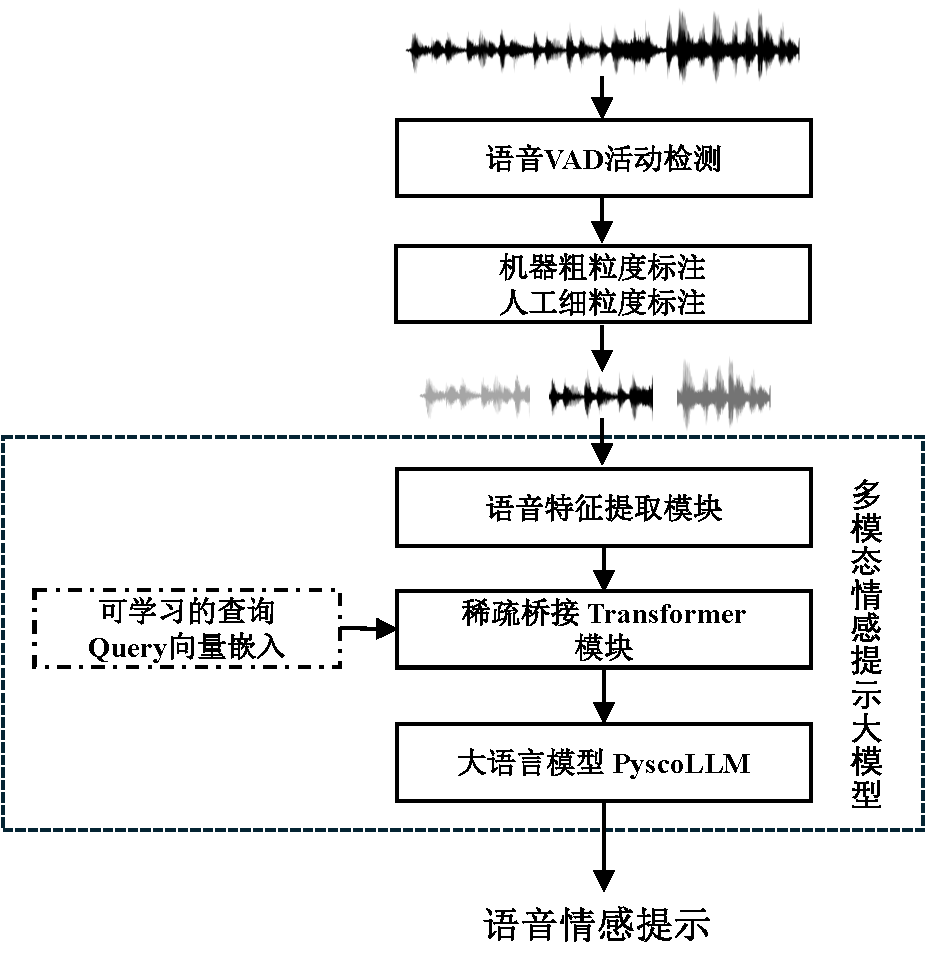
\includegraphics[width=0.8\textwidth]{work2-workflow.pdf}
  \caption{多模态情感描述大模型 SEMO-LLM 整体流程图}
  \label{fig:work2-workflow}
\end{figure}

\begin{figure}[ht]
  \centering
  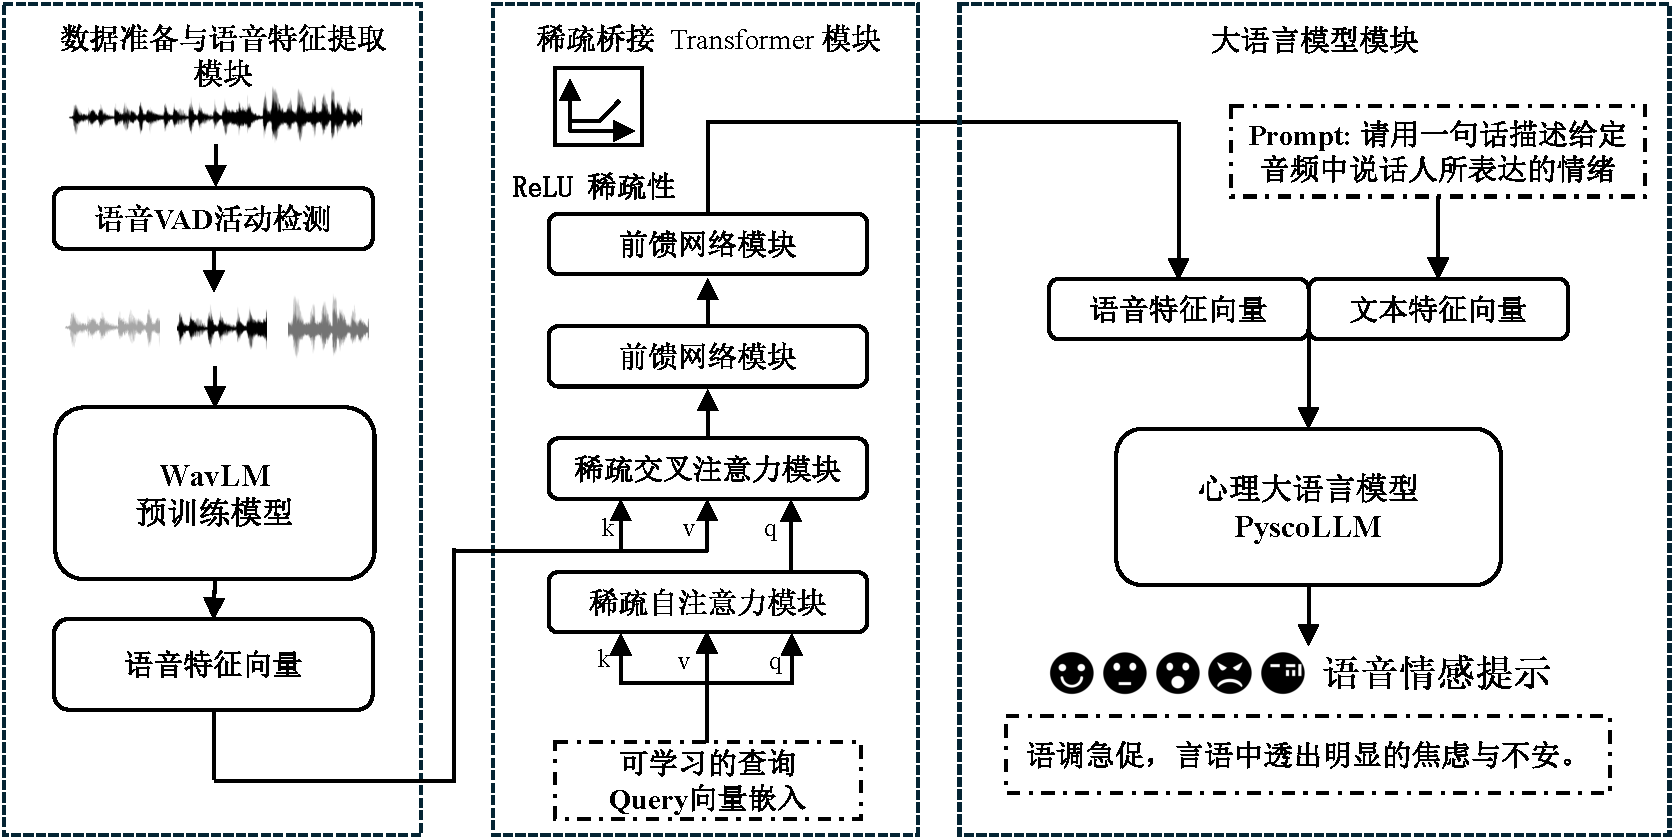
\includegraphics[width=1\textwidth]{work2-architecture.pdf}
  \caption{多模态情感描述大模型 SEMO-LLM 整体结构}
  \label{fig:work2-architecture}
\end{figure}

\subsection{语音处理模块}

语音处理模块主要完成原始语音数据的预处理、分割与情感特征提取,具体分为以下三个步骤:

\textbf{1. 数据预处理与分割}

从语音对话场景中获取原始语音数据 $S = \{s_1, s_2, ..., s_n\}$,每段数据 $s_i$ 表示包含情感信息的语音信号。
对原始数据进行降噪和归一化操作,消除背景噪音的干扰,确保数据质量的一致性。
使用语音活动检测(VAD)算法,通过计算短时能量 $E(t)$ 并设定阈值 $\theta$,将语音信号划分为语音活动区与静音区并根据停顿端点分割出高保真语音片段集合 $P = \{p_1, p_2, ..., p_m\}$。  

\textbf{2. 情感标签生成}

粗粒度情感标签利用情感分类模型 $f_{\text{classify}}$ 计算每个语音片段 $p_k$ 的情感类别概率分布,并分配基本情感类别(如愉快、愤怒、悲伤等),并根据语音转录文本生成粗粒度情感描述。细粒度情感标签通过人工标注将粗粒度情感标签细化为更加具体的情感表达(如“略带愤怒的愉快”或“轻微焦虑的平静”),生成高质量的细粒度情感标签集合。  

\textbf{3. 语音特征提取}

基于 WavLM 预训练模型对预处理后的语音片段进行特征提取,得到多层次的语音特征向量 $V$。WavLM模型通过门控相对位置偏置的 Transformer 结构,能够有效捕捉语音的声学特征,包括音高、语速、语调等信息,为后续情感识别提供关键输入。经过处理与特征提取,语音处理模块输出一组带有情感标签的高质量语音特征样本,为模型的训练和优化提供坚实的数据基础。

\subsection{稀疏桥接 Transformer 模块}

稀疏桥接 Transformer 模块是实现语音与文本特征对齐的核心组件,稀疏注意力如图 \ref{fig:sparse-attention} 所示,通过稀疏自注意力和稀疏交叉注意力机制,对语音特征向量与文本向量进行融合与对齐,具体包括以下步骤:  

\begin{figure}[ht]
  \centering
  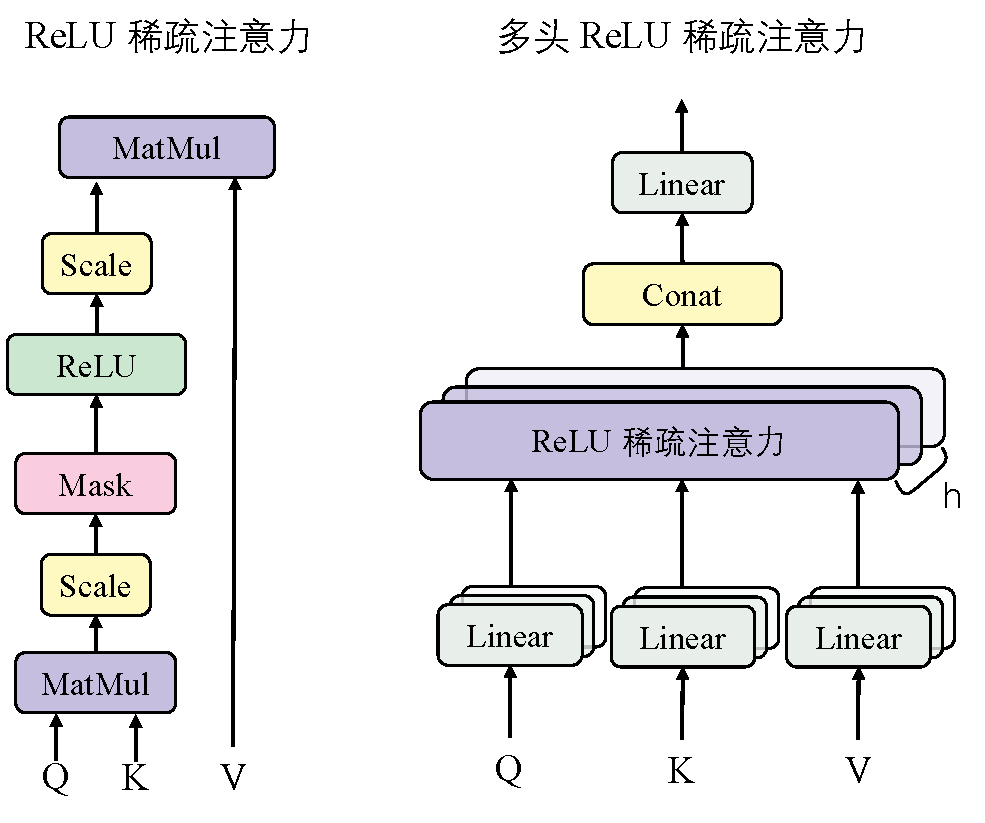
\includegraphics[width=0.8\textwidth]{sparse-attention.pdf}
  \caption{稀疏注意力机制}
  \label{fig:sparse-attention}
\end{figure}

\textbf{1. 稀疏自注意力机制}

定义一个随机初始化的可学习查询向量 $Q_{\text{query}}$,作为额外的输入特征向量。$Q_{\text{query}}$ 与原始语音特征向量 $V$ 通过稀疏自注意力机制进行匹配,提取情感相关的语音特征向量 $A_{\text{self}}$。公式表示为:
\begin{equation}
    A_{\text{self}} = L^{-1} \text{ReLU} \left( \frac{Q W_q (Q W_k)^T}{\sqrt{d_k}} \right) Q W_v,
\end{equation}
其中,$W_q, W_k, W_v$ 为稀疏自注意力机制的查询、键和值矩阵,$L$ 可学习查询向量的序列长度,可以在缩放性方面匹配传统的 Softmax 操作,同时计算代价比 Softmax 更便宜。

\textbf{2. 稀疏交叉注意力机制}

将 $A_{\text{self}}$ 作为查询,原始语音特征向量 $V$ 作为键和值,通过交叉注意力机制生成最终的对齐后的语音情感向量 $A_{\text{cross}}$。公式表示为:
\begin{equation}
    A_{\text{cross}} = L^{-1} \text{ReLU} \left( \frac{A_{\text{self}} W_q (V W_k)^T}{\sqrt{d_k}} \right) V W_v.
\end{equation}

\textbf{3. 语音与情感描述对比学习}

由于语音表示的高维度和冗余性,语音特征包含丰富的信息,如内容和背景噪声,其中只有一部分与情绪相关。为了减轻心理大模型处理语音特征的复杂性,本文希望稀疏桥接 Transformer 模块能够够提取与语音情感描述高度相关的特征,从而减少语音特征和文本模态之间的差距。本文将语音引入到稀疏桥接 Transformer 中,得到 Q-Embedding $Q_A$;将情感描述文本引入到预训练的 Bert 文本编码器中,得到 C-Embedding $Q_C$ 。通过对比学习,使得 Q-Embedding 和 C-Embedding 在语义空间中更加接近,从而提升情感描述生成的准确性。

为了减少在对比学习中情感相似的负样本的影响,本文将数据集根据不同情感标签类别进行划分为 $N$ 个类别。这样做可以保证不同类别之间语音情感字幕的差异性,从而增强模型在学习过程中的区分能力。在每次训练步骤中,本文从每个类别中选择 $K$ 个语音-提示对,确保对于每个 $Q_A$, $Q_C$ 对,有 $K - 1$ 个相似的情感描述,以及 $(N - 1)K$ 个不相似的情感描述作为负样本,从而构建对比学习的损失函数如下:
\begin{equation}
\begin{aligned}
  \mathcal{L}_{contrastive} = & \sum_{i=1}^{NK} \left[ w_1(1 - sim(Q_{A_i}, Q_{C_i})) + w_2 \sum_{j=1}^{K-1} (1 - sim(Q_{A_i}, Q_{C_{ij}})) \right. \\
  & \left. + w_3 \sum_{j=1}^{(N-1)K} \text{ReLU}(sim(Q_{A_i}, Q_{C_{ij}}) - \mu) \right],
\end{aligned}
\end{equation}
其中,N 表示情感类别标签数量,K 表示每个类别选择的语音-提示对,$sim$ 表示两个向量之间的余弦相似度,$w_1, w_2, w_3$ 分别表示不同的权重系数,$\mu$ 表示负样本的阈值。通过最小化 $L_{\text{contrastive}}$,能够很好地优化桥接 Transformer 模块,提升语音和文本模态之间的信息融合能力。

\subsection{大模型情感描述生成模块}

大模型情感描述生成模块基于第三章所训练的心理大语言模型作为底座,通过多模态融合特征生成情感描述文本。该模块的核心目标是基于输入的语音特征和文本提示词,通过自回归解码生成符合语音语境的情感描述信息。具体过程如下:

\textbf{1. 多模态特征输入}

将经过稀疏桥接 Transformer 得到的语音特征向量和精心设计的文本提示词(例如“请用一句话描述音频中的情感表现”)经过词嵌入层得到的文本特征在特征纬度上进行对齐拼接得到 $I_{\text{input}}$,输入到第三章所训练的心理大模型底座。

\textbf{2. 文本解码生成情感描述}

心理大模型自回归解码过程包括三个步骤:(1)在生成初始状态时,模型根据输入特征 $I_{\text{input}}$ 计算起始分布;(2)模型以生成的每个单词或标记作为下一步输入,逐步预测下一个单词,直到生成结束标记或满足生成条件;(3)最终输出完整的情感描述文本 $Y$,具体公式表示为:
\begin{equation}
   Y = \arg\max_{y} P(y \mid I_{\text{input}}),
\end{equation}
其中,$P(y \mid I_{\text{input}})$ 表示基于多模态输入特征生成文本 $y$ 的概率分布。

\textbf{3. 优化与损失函数}

为了优化生成文本的质量,本模块采用自回归的交叉熵损失函数 $L_{\text{CE}}$,衡量生成的情感描述文本与参考文本之间的匹配程度。损失函数定义如下:
\begin{equation}
    L_{\text{CE}} = - \sum_{t=1}^{T} \log P(y_t \mid y_{<t}, I_{\text{input}}),
\end{equation}
其中,$T$ 表示生成序列的长度;$y_t$ 表示第 $t$ 个生成单词;$y_{<t}$ 表示生成到第 $t-1$ 步的所有前缀。通过最小化 $L_{\text{CE}}$,模型能够逐步优化生成过程,提升情感描述文本的流畅性和语义准确性。

\section{实验与分析}

\subsection{数据集介绍}

为了验证 SEMO-LLM 模型的性能,以及构建多模态情感描述大模型 SEMO-LLM 的训练数据集,本研究基于 IEMOCAP 和 MELD 语音情感数据集进行情感描述的标注,在标注好的数据集上进行训练与评估 SEMO-LLM 模型。

IEMOCAP \cite{Busso_Bulut_Lee_Kazemzadeh_Mower_Kim_Chang_Lee_Narayanan_2008} 是一个用于双人对话情感识别的语料库,包含多个双人对话视频,每个视频展示了一段对话。对话的表演者包括10名参与者(5男5女),这些对话被划分为5个会话(session),每个会话中,一对男女演讲者会参与不同的对话场景。每段对话由多个话语构成,每个话语都被标注为以下情感之一:中性(neutral)、快乐(happiness)、悲伤(sadness)、愤怒(anger)、沮丧(frustrated)或兴奋(excited)。该数据集的训练集、验证集和测试集分别包含4810条、1000条和1523条语音样本。

MELD \cite{Poria_Hazarika_Majumder_Naik_Cambria_Mihalcea_2019} 是一个源自电视剧《老友记》的多人对话情感识别数据集,数据来源于剧中的对话片段。该数据集包含七种情感类别:中性(neutral)、快乐(happiness)、惊讶(surprise)、悲伤(sadness)、愤怒(anger)、厌恶(disgust)和恐惧(fear)。MELD数据集的训练集包含9989条样本,验证集1109条样本,测试集2610条样本。

在标注流程中,首先利用预训练的 Qwen2-Audio-7B-Instruct 语音大模型对语音文本进行预标注,这一阶段主要生成文本形式的情感描述,描述语音中的核心情绪特征,包括情感类别和情感强度。随后,标注人员参考转录文本以及机器生成的情感描述文本进行人工修正。在修正过程中,标注人员通过反复聆听语音样本,并结合转录文本内容与情感标签,对初始生成的情感描述进行精细化调整。修正后的情感描述综合考虑了语音的情绪特征、音量变化以及语速信息,以确保标注结果的准确性和一致性。

为进一步确保数据集的高质量,本文对标注流程进行了严格的质量控制。例如,在标注规则制定阶段,标注团队通过对 50 条示例语音样本的独立标注,开展集中讨论,明确情感标注的标准化规则。标注过程中,每段语音均经过多名标注人员的独立评估,以减少个人主观偏差。此外,本文随机抽取每 100 条标注中的 5 条语音样本,交由其他标注人员进行一致性检查,从而保证整体标注的可靠性和高标准。

\subsection{实验设置与评价指标}

\textbf{1. 实验环境设置}

本章提出的 SEMO 模型使用 PyTorch 深度学习框架以及 Huggingface Transformers 框架实现,具体的硬件配置和软件配置如表 ~\ref{tab:work2-实验环境配置} 所示。

\begin{table}
  \centering
  \caption{SEMO-LLM 实验环境配置}
  \label{tab:work2-实验环境配置}
  \begin{tabular}{cc}
    \toprule
    配置项 & 版本信息 \\
    \midrule
    CPU & Intel(R) Xeon(R) Gold 6326 CPU @ 2.90GHz \\
    GPU & NVIDIA A800 Tensor Core GPU \\
    操作系统 & Ubuntu 22.04 LTS \\
    CUDA 版本 & 12.4 \\
    Python & 3.11.9 \\
    PyTorch & 2.4.0 \\
    Huggingface Transformers & 4.46.1 \\
    \bottomrule
  \end{tabular}
\end{table}

\textbf{2. 实现细节}

本文提出的 SEMO-LLM 模型结构主要包括三个部分:语音特征提取模块 WavLM、稀疏桥接 Transformer 模块和大模型提示生成模型 PsycoLLM。

语音特征提取模块 WavLM 使用预训练的 WavLM-Large 模型,该模型在大规模的语音数据集上进行预训练,能够有效提取语音特征。WavLM-Large 模型的输入为原始音频信号,经过特征提取后输出为 1024 维度的语音特征向量。WavLM-Large 模型基于 Transformer 架构,包含 24 层 Transformer 编码器,每一层的隐藏层维度为 1024,通过自注意力机制处理音频序列中的上下文信息。这些层在预训练过程中,通过大规模语音数据学习了丰富的音频表示,能够有效捕捉语音信号中的语音、情感等多种信息特征。同时,为了能够对齐 WavLM 和稀疏桥接 Transformer 模块的特征维度,本文将 WavLM-Large 模型的输出维度经过可学习的线性层调整为 768。

稀疏桥接 Transformer 模块主要包括稀疏自注意力和稀疏交叉注意力机制,用于对齐语音特征向量和文本特征向量。它的参数设置采用标准的 Transformer 模型参数设置,包括 12 层 Transformer 编码器,每一层的隐藏层纬度为 768,最后接一个两层线性层将输出纬度调整为情感描述大语言模型的词嵌入输入维度,这里 PsycoLLM 模型为 14B 参数大小,特征维度为 5120。

大模型情感描述生成模块 PsycoLLM 使用第三章训练的心理大语言模型 PsycoLLM 作为底座,其基于 Qwen2-14B-Instruct 模型在第三章所构建的数据集上进行训练,能够生成符合语音语境的情感描述文本。因此 PsycoLLM 模型的文本的词表大小为 152064,包括 48 层 Transformer 解码器,采用分组多查询注意力机制(Grouped Multi-Query Attention,GQA),查询头为 40,键值头为 8,隐藏层纬度为 5120,模型参数大小为 14B。

模型的训练过程包括两个阶段,第一个阶段对稀疏桥接 Transformer 进行对比学习训练,使桥接模块在第二阶段初始阶段拥有更好的对齐语音到文本特征的能力。训练阶段包括 20 个 epoch,训练过程中,每个 batch 的大小为 256,并且采用 AdamW 优化器,该优化器能够通过引入权重衰减来稳定训练过程,并有效防止过拟合。实验采用基础学习率为 1e-4 的线性衰减调度策略;对比损失函数的超参数配置为 $w_1 = 1.0, w_2 = 0.5, w_3 = 0.5, \mu = 0.5$。

第二阶段训练 PsycoLLM 模型,在模型训练阶段,批处理规模(batch size)设置为 32,初始学习率(learning rate)固定为 1e-5,优化策略选用 AdamW,训练周期数(epochs)为 10。训练过程中,冻结语音特征提取器的参数,只训练稀疏桥接 Transformer 模块和 PsycoLLM 模型的参数,稀疏桥接 Transformer 模块采用全量参数训练,PsycoLLM 模型采用 LoRA 策略进行训练,LoRA rank 设置为 8。整个训练过程在一张 NVIDIA A800 Tensor Core GPU 上进行。

\textbf{3.评价指标}

在情感描述任务中,每条数据样本包含三个要素:$\mathcal{T}$:表示语音样本;$\mathcal{E}$:语音对应的情感标签,用于指示语音中表达的主要情感类型;$\mathcal{C}$:标准情感描述文本,综合文本和情感标签生成的完整参考答案。

模型根据输入的 $\mathcal{T}$ 和 $\mathcal{E}$ 生成情感描述文本 $\mathcal{O}$。为评价生成的 $\mathcal{O}$ 的质量,本文采用以下文本生成任务的标准评估指标和语义相似性指标:(1)BLEU-1:计算1-gram(单个词)的精确度,即机器翻译中有多少个词与参考文本匹配;(2)BLEU-4:计算4-gram(四个连续的词)重叠的精确度,用来更全面地评估机器翻译的质量;(3)ROUGE-L:基于模型输出与参考摘要之间的最长公共子序列(LCS)匹配,衡量生成内容对关键信息的覆盖程度;(4)CIDEr:该指标旨在评估文本生成模型的综合性能,其核心方法是基于术语频率-逆文档频率(TF-IDF)的加权计算,通过量化生成内容与参考文本之间的一致性来实现;(5)SPICE:该评估指标利用语义场景图计算 F-score,以衡量生成文本与参考文本的匹配程度。具体而言,首先通过依存关系解析将文本转换为句法依赖树,随后将其映射为场景图表示,最终基于该表示计算 F-score 值。

标准评估指标主要关注词级别的匹配。为了更有效地在句子级别评估两个中文情感字幕的相似性,本文结合上述标准,进一步采用了 BERTScore 进行句子相似性的评估。BERTScore 评估指标依托于 BERT 预训练语言模型,通过度量待评估文本与标准参考在词向量空间的余弦相似性,进而衡量两者间的语义匹配度。

\subsection{对比实验与分析}

为了验证本章提出的模型效果,本文选取了多种基线模型进行对比实验,各个基线模型的详细介绍如下所示:

Qwen2-Audio-7B-Instruct:Qwen 系列的通用音频大模型。 Qwen2-Audio 能够接受各种音频信号输入并执行音频分析或有关语音说明的直接文本响应。包括两种不同的音频交互模式,如语言聊天和音频分析。语音聊天指用户可以在没有文本输入的情况下自由地与 Qwen2-Audio 进行语音互动;音频分析指用户可以在交互期间提供音频和文本说明。在对比实验中,本文主要借助 Qwen2-Audio-7B-Instruct 模型的语音分析能力,直接给定情感语音,分析生成情感描述文本。

WavCaps:在一个大规模的弱标记数据集上训练的 HTSAT-BART 模型,该模型在 AudioCaps 上实现了最先进的性能。本文直接将 WavCaps 的 HTSAT-BART 模型结构应用于情感描述生成任务,即语音编码器使用 HTSAT 模型,文本解码器使用 BART 模型,桥接网络使用线性层。

SECap:基于音频编码器 HuBERT 和 LLaMA 大语言模型的情感描述生成模型。该模型通过音频编码器 HuBERT 提取音频特征,然后通过 Q-Former 将音频特征与文本特征对齐,最后通过 LLaMA 解码器生成情感描述文本。

本章所提出的方法在模型结构上与 WavCaps 以及 SECap 不同的是,音频编码器使用了 WavLM-Large,WavLM-Large 的特征提取能力相较于 HTSAT 和 HuBERT 效果更好;桥接网络稀疏桥接 Transformer 模块,与 Q-Former 使用的标准 Softmax 注意力不同,稀疏桥接 Transformer 模块引入了 ReLU 替代 SoftMax 作为稀疏自注意力和稀疏交叉注意力机制,ReLU 注意力的一大优势是能在序列长度维度上实现并行化,其所需的收集操作比 softmax 注意力更少。文本解码器使用了本文第三章所训练的心理大模型底座,能够更好地生成情感描述文本。在带有 IEMOCAP 和 MELD 数据集的情感描述生成任务中,本文对比了上述基线模型的性能,通过 BLEU-1、BLEU-4、ROUGE-L、CIDEr、SPICE 和 BERTScore 等多项指标进行评估,对比结果如表和表 \ref{tab:IEMOCAP对比实验} 和表 \ref{tab:MELD对比实验} 所示。

\begin{table}
  \centering
  \caption{IEMOCAP 数据集对比实验}
  \label{tab:IEMOCAP对比实验}
  \begin{tabular}{ccccccc}
    \toprule
    模型 & BLEU-1 & BLEU-4 & ROUGE-L & CIDEr & SPICE & BERTScore \\
    \midrule
    WavCaps & 29.32 & 5.78 & 25.47 & 28.49 & 5.35 & 67.26 \\
    Qwen2-Audio & 30.48 & 6.89 & 25.94 & 28.31 & 6.12 & 69.64 \\
    SECap & 34.12 & 7.02 & 26.43 & 30.19 & 6.47 & 70.45 \\
    Our model & 35.67 & 7.45 & 28.71 & 32.05 & 6.86 & 71.82 \\
    \bottomrule
  \end{tabular}
\end{table}

\begin{table}
  \centering
  \caption{MELD 数据集对比实验}
  \label{tab:MELD对比实验}
  \begin{tabular}{ccccccc}
    \toprule
    模型 & BLEU-1 & BLEU-4 & ROUGE-L & CIDEr & SPICE & BERTScore \\
    \midrule
    WavCaps & 26.39 & 5.20 & 22.92 & 25.64 & 4.81 & 60.89 \\
    Qwen2-Audio & 28.94 & 6.17 & 23.35 & 26.98 & 5.51 & 66.67 \\
    SECap & 31.72 & 6.72 & 24.89 & 27.17 & 6.14 & 66.91 \\
    Our model & 32.12 & 6.88 & 26.38 & 29.11 & 6.58 & 67.64 \\
    \bottomrule
  \end{tabular}
\end{table}

实验结果表明,本文提出的情感描述生成模型在所有评估指标上均取得了优于基线模型的表现,进一步证明了本文方法的有效性。从 \textbf{IEMOCAP} 数据集 的实验结果来看,本文模型在 BLEU-1 和 BLEU-4 指标上分别达到 \textbf{35.67} 和 \textbf{7.45},相较于 SECap(34.12 和 7.02)、Qwen2-Audio(30.48 和 6.89)以及 WavCaps(29.32 和 5.78)均有不同程度的提升,表明本文方法在情感描述文本的 n-gram 匹配度方面表现更优。此外,在 ROUGE-L 指标上,本文模型取得 \textbf{28.71},较 SECap(26.43)和 Qwen2-Audio(25.94)明显提升,说明生成文本的覆盖度更广、与参考文本的相似度更高。同时,在衡量文本质量的 CIDEr 和 SPICE 指标上,本文方法分别取得 \textbf{32.05} 和 \textbf{6.86},均超越所有基线模型,显示了在描述完整性和文本多样性上的优势。最后,BERTScore 方面,本文模型达到 \textbf{71.82},相比于 SECap(70.45)、Qwen2-Audio(69.64)和 WavCaps(67.26),进一步证明了模型在生成语义质量上的提升。

在 \textbf{MELD} 数据集 上,本文方法同样取得了领先的结果。BLEU-1 和 BLEU-4 分别达到 \textbf{32.12} 和 \textbf{6.88},超越 SECap(31.72 和 6.72)、Qwen2-Audio(28.94 和 6.17)以及 WavCaps(26.39 和 5.20),显示出更强的短语匹配能力。在 ROUGE-L 方面,本文模型取得 \textbf{26.38},相比于 SECap(24.89)和 Qwen2-Audio(23.35)有明显优势,说明生成的文本与真实参考文本的整体相似度更高。此外,在 CIDEr 和 SPICE 方面,本文模型的得分分别为 \textbf{29.11} 和 \textbf{6.58},高于所有基线模型,表明其在生成丰富性和文本结构上具有更好的表现。而在 BERTScore 指标上,本文方法达到 \textbf{67.64},相比于 SECap(66.91)、Qwen2-Audio(66.67)和 WavCaps(60.89),进一步证明了本文方法能够生成更符合语义的情感描述文本。

\subsection{消融实验与分析}

为了评估本文方法模型结构的有效性,在 IEMOCAP 和 MELD 数据集上进行了消融实验,具体分为考虑不同的音频编码器、桥接网络和文本解码器组合:(1)音频编码器,包括 HuBERT 和 WavLM 两种语音预训练模型,用于从音频信号中提取特征;(2)桥接网络,使用了 Linear、Q-Former 和本文提出的稀疏桥接 Transformer 架构(记为 Sparse Q-Former),将音频特征与文本特征对齐;(3)文本编码器,除了基于第三章所训练的心理大模型底座,本章还考虑采用原始的 Qwen2.5-14B 模型底座作为文本解码器,通过解码文本特征来分析和生成情感描述。

\begin{table}
  \centering
  \caption{IEMOCAP 数据集消融实验}
  \label{tab:IEMOCAP 消融实验}
  \begin{tabular}{ccccc}
      \toprule
      音频编码器 & 桥接网络 & 文本编码器 & BERTScore \\
      \midrule
      HuBERT & Linear & Qwen2.5-14B & 68.12 \\
      HuBERT & Q-Former & Qwen2.5-14B & 69.45 \\
      HuBERT & Sparse Q-Former & Qwen2.5-14B & 70.12 \\
      WavLM & Sparse Q-Former & Qwen2.5-14B & 70.49 \\
      WavLM & Q-Former & Our model & 71.42 \\
      WavLM & Sparse Q-Former & Our model & 71.82 \\
      \bottomrule
  \end{tabular}
\end{table}

\begin{table}
  \centering
  \caption{MELD 数据集消融实验}
  \label{tab:MELD 消融实验}
  \begin{tabular}{ccccc}
      \toprule
      音频编码器 & 桥接网络 & 文本编码器 & BERTScore \\
      \midrule
      HuBERT & Linear & Qwen2.5-14B & 63.86 \\
      HuBERT & Q-Former & Qwen2.5-14B & 63.92 \\
      HuBERT & Sparse Q-Former & Qwen2.5-14B & 64.20 \\
      WavLM & Sparse Q-Former & Qwen2.5-14B & 65.34 \\
      WavLM & Q-Former & Our model & 66.98 \\
      WavLM & Sparse Q-Former & Our model & 67.64 \\
      \bottomrule
  \end{tabular}
\end{table}

消融实验结果如表~\ref{tab:IEMOCAP 消融实验}和表~\ref{tab:MELD 消融实验}所示,各组件对最终性能均有显著影响。首先,从 音频编码器 的选择来看,WavLM 在所有实验配置下均优于 HuBERT。这表明 WavLM 在情感特征提取方面更加有效,能够提供更具判别力的音频特征,从而提升最终的 BERTScore 结果。例如,在 IEMOCAP 数据集上,HuBERT 结合 Sparse Q-Former 和 Qwen2.5-14B 作为文本解码器时,BERTScore 达到 70.12,而更换为 WavLM 后,该分数提升至 70.49。此外,在 MELD 数据集上,同样的结构下,HuBERT 取得 64.20,而 WavLM 提高至 65.34,进一步验证了 WavLM 在跨模态情感识别任务中的优势。

其次,桥接网络的影响也较为明显。Linear 作为最简单的桥接方式,在所有实验设置中均表现最差,例如 IEMOCAP 数据集上 HuBERT + Linear + Qwen2.5-14B 仅取得 68.12,明显低于更复杂的 Q-Former 和 Sparse Q-Former 结构。这说明简单的线性映射不足以充分对齐音频和文本特征,而基于 Transformer 机制的 Q-Former 能够更好地建模跨模态关系。因此,在相同音频编码器和文本编码器的情况下,Linear 到 Q-Former 的提升较为显著,如 IEMOCAP 数据集上 HuBERT + Q-Former + Qwen2.5-14B 由 68.12 提高到 69.45。此外,Sparse Q-Former 进一步提升了性能,相较于普通 Q-Former 在所有设置下均有稳定提升,如 WavLM + Sparse Q-Former + Qwen2.5-14B 在 IEMOCAP 数据集上达到 70.49,而 WavLM + Q-Former + Qwen2.5-14B 仅为 70.12,证明了本文提出的 Sparse Q-Former 结构在跨模态对齐上的有效性。

最后,文本编码器的选择对最终结果起到了关键作用。从 MELD 数据集的实验结果来看,相较于 Qwen2.5-14B,本文基于心理大模型优化的文本解码器在所有实验配置下均有明显提升。例如,在 WavLM + Sparse Q-Former 结构下,更换为本模型后,BERTScore 从 65.34 提高到 67.64。这说明结合心理健康知识微调的文本模型能够更有效地捕捉情感相关信息,提升跨模态情感分析的效果。

类似 SECap 方法,本文针对稀疏桥接 Transformer 模块进行了对比学习,通过对比学习,可以让稀疏桥接 Transformer 模块在初始阶段更好地对齐音频和文本特征,以提升情感描述生成的准确性。本文考虑了是否使用对比学习的情况下的模型性能,以及在语音情感描述大模型训练过程中冻结稀疏桥接 Transformer 模块的效果,实验结果如表 \ref{tab:桥接模块在 IEMOCAP 数据集的消融实验} 和表 \ref{tab:桥接模块在 MELD 数据集的消融实验} 所示。

\begin{table}
  \centering
  \caption{桥接模块在 IEMOCAP 数据集的消融实验}
  \label{tab:桥接模块在 IEMOCAP 数据集的消融实验}
  \begin{tabular}{cccc}
      \toprule
      模型 & 对比学习 & 冻结参数 & BERTScore \\
      \midrule
      SECap & × & × & 69.46 \\
      SECap & √ & × & 70.45 \\
      SECap & √ & √ & 62.89 \\
      Our model & × & × & 69.84 \\
      Our model & √ & × & \textbf{71.82} \\
      Our model & √ & √ & 64.78 \\
      \bottomrule
  \end{tabular}
\end{table}

\begin{table}
  \centering
  \caption{桥接模块在 MELD 数据集的消融实验}
  \label{tab:桥接模块在 MELD 数据集的消融实验}
  \begin{tabular}{cccc}
      \toprule
      模型 & 对比学习 & 冻结参数 & BERTScore \\
      \midrule
      SECap & × & × & 65.87 \\
      SECap & √ & × & 66.91 \\
      SECap & √ & √ & 63.04 \\
      Our model & × & × & 66.12 \\
      Our model & √ & × & \textbf{67.64} \\
      Our model & √ & √ & 63.78 \\
      \bottomrule
  \end{tabular}
\end{table}

首先,本文观察到使用对比学习可以显著提升模型性能。在 IEMOCAP 数据集上,采用对比学习的 SECap 模型(第二行)相较于不使用对比学习的版本(第一行)在 BERTScore 上提高了约1.0点。而在本文的模型上,使用对比学习的效果更加明显,BERTScore 从 69.84 提升至 71.82,达到了最高性能。

进一步地,冻结稀疏桥接 Transformer 模块的参数对模型性能的影响也值得关注。在 IEMOCAP 数据集上,冻结该模块后,模型的 BERTScore 显著下降,从 71.82 降至 64.78,表明冻结该模块会导致性能的显著退化。这一趋势在 MELD 数据集上也得到了验证,冻结模块参数后的 BERTScore 从 67.64 降至 63.78,虽然下降幅度相对较小,但仍然明显低于不冻结参数的情况。

从这些实验结果可以得出,使用对比学习能够有效提升稀疏桥接 Transformer 模块在音频和文本特征对齐上的表现,从而提高情感描述生成的准确性。然而,冻结该模块的参数可能会限制模型的学习能力,导致性能下降。总体来看,稀疏桥接 Transformer 模块的动态更新对提升模型的情感识别能力至关重要。

\subsection{可视化展示与分析}

为了更直观地展示本文提出的模型在情感描述生成任务中的性能,本文选取了 IEMOCAP 数据集中的一些测试样本进行可视化展示,展示了不同模型生成的情感描述文本。具体来说,本文选取了一些语音测试样本,分别使用 Qwen2-Audio、SECap 和本文提出的模型生成情感描述文本,展示了三种模型生成的情感描述文本。为了更直观地展示,本文挑选了语音对应的视频人物图片序列进行展示,可以直观看到人物的情绪变化。具体展示如图 \ref{fig:work2-example} 所示,

\begin{figure}[ht]
  \centering
  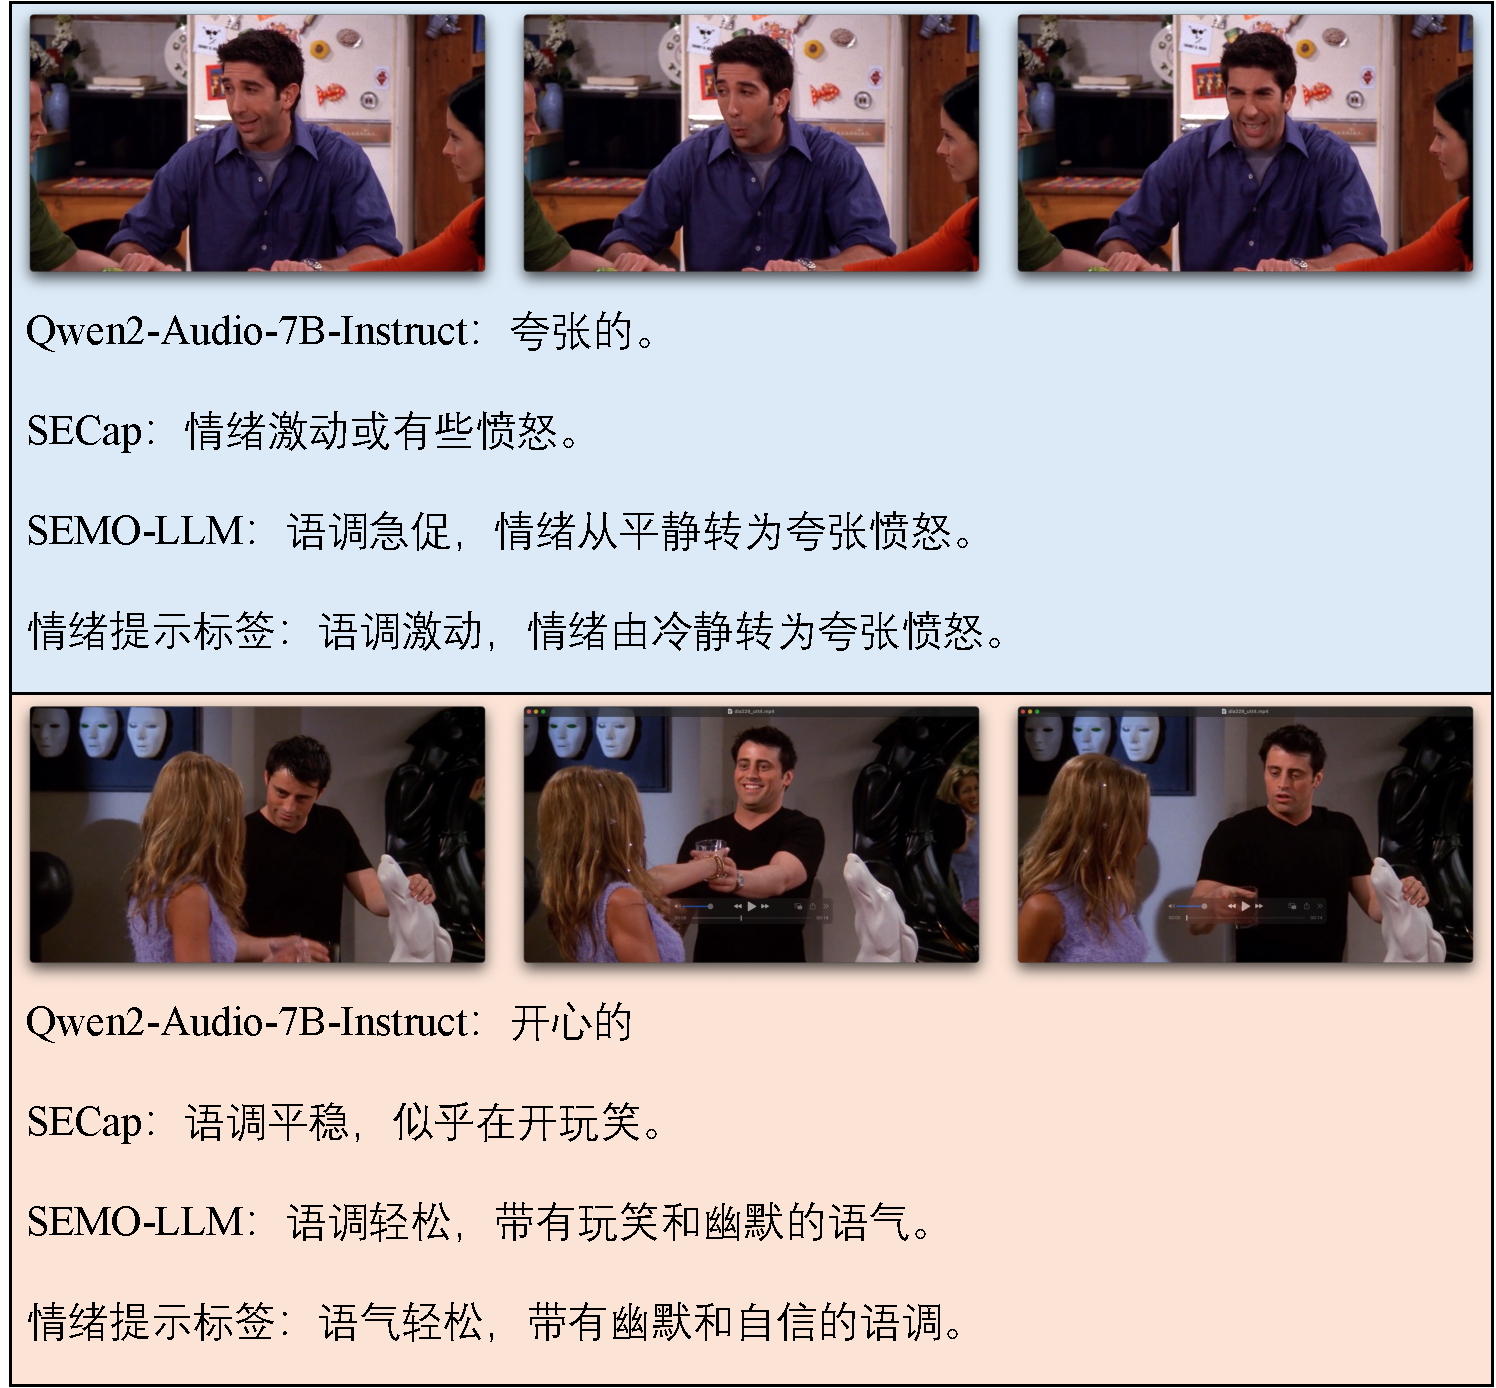
\includegraphics[width=1\textwidth]{work2-example.pdf}
  \caption{可视化展示示例}
  \label{fig:work2-example}
\end{figure}

通过可视化展示结果可以看到,本文提出的模型生成的情感描述文本更加准确和丰富,能够更好地描述语音中的情感特征。例如,在第一个示例中,Qwen2-Audio 生成的情感描述文本为“夸张的”,描述较为单一,而 SECap 生成的情感描述文本为“情绪激动或有些愤怒”,虽然描述稍微准确,但是缺乏情感变化的描述。而本文提出的模型生成的情感描述文本为“语调轻松,情绪从平静转为夸张愤怒”,不仅描述了情绪状态,还描述了情感强度变化,更加全面地表达了语音中的情感特征。

\section{本章小结}

本章提出了一种面向语音交互场景的多模态情感描述大模型 SEMO-LLM,通过语音处理模块、稀疏桥接 Transformer 模块和大语言模型情感描述生成模块的协同设计,实现了语音与文本模态的深度融合和高效情感描述生成。模型在 IEMOCAP 和 MELD 数据集上进行训练与评估,通过严格的数据标注与质量控制,构建了高质量的情感描述数据集。实验结果表明,本文提出的模型在情感描述生成任务中的多项指标上均优于基线模型,尤其是在 SIM 和 BERTScore 等语义相似性指标上的表现更为突出,为实际应用场景中语音情感识别与反馈的提升提供了重要支持。
